
\emptysection{TD 1A Algorithmique}{Initiation aux tableaux\\Durée : 2H30}
%%
\begin{center}
  \Large\bf Communication numérique et sobriété
\end{center}

\noindent\rule{\linewidth}{.6pt}

\bigskip

Source : les estimations environnementales proviennent de l'Ademe (\url{impactco2.fr}).

\oldsection*{Contexte}

Afin de regagner en souveraineté sur le secteur stratégique des réseaux sociaux pour collégiens, votre société a pour mission de développer une nouvelle application de communication rapide et
de haut niveau intellectuel~: Bikbok.
%GA BikBook? 
%% et surtout sensibilisant l'utilisateur aux problèmes d'environnement en affichant l'empreinte carbone du message
%% [DLB] Oui mais comment faire ? L'impact d'un seul message sera tellement ridicule...
\medskip

Votre équipe est chargée d'écrire un démonstrateur capable d'\textbf{envoyer} les messages. Une autre équipe se charge de la réception et de l'affichage. Les types des messages sont :
texte, vocal, photo, ou vidéo.
Pour la démonstration prévue dans deux semaines, le message envoyé sera, par exemple :

\medskip
\centerline{\hword{\ Pour ce soir (@kollok) : pâtes ou pizza ?\ }}
\medskip

Malgré le caractère confidentiel du message, il est envoyé en clair -- sans être chiffré. Ce message comprend 41 caractères, dure 3 secondes en vocal et en vidéo.
\oldsection{Message texte}

$\star$ Écrire un petit programme qui~:

\begin{itemize}[itemsep=0.2ex]
\item[$\cdot$] Utilise l'acteur Texte ci-après ;
\item[$\cdot$] Récupère le message tapé par l'utilisateur ;
\item[$\cdot$] Compte les destinataires mentionnés dans le message avec '@' (e.g. @Estelle, @Leo, @Thomas). Une fonction auxiliaire sera bienvenue.
\item[$\cdot$] Envoie le message.
\end{itemize}
Une chaîne de caractères (String) est un tableau~:

\begin{center}
  \begin{tabular}{c|cccccccccccccccccccccccccc}
{\large\strut}   Indice & 1 & 2 & 3 & 4 & 5 & 6 & 7 & 8 & 9 & 10 & 11 & 12 & ... \\[1ex]
{\large\strut}   Cellule & \cell{P} & \cell{o} & \cell{u} & \cell{r} & \cell{\ } & \cell{c} & \cell{e} & \cell{\ } & \cell{s} & \cell{o} & \cell{i} & \cell{r} & ... \\
  \end{tabular}
\end{center}

\lstinputlisting[language=Ada]{Ada/texte.ads}

\subsection*{Coût environnemental}

La taille du message se mesure en octets : il faut maximum deux octets par caractère.
Estimons l'ordre de grandeur de l'impact sur le dérèglement climatique (i.e. le coût en g-eCO2, g équivalent CO2).

\begin{itemize}[itemsep=0.2ex]
\item[$\cdot$] Combien de messages envoyez-vous par an ? (à 10.000 près)
\item[$\cdot$] Coût de la transmission : 10~g-eCO2 par Go (grammes équivalent~CO2 par giga-octets).\\
  {\small Source : Ademe, d'après \url{negaoctet.org}}
\item[$\cdot$] Exprimer le coût annuel dans une unité étudiant-compatible~: l'ecafé (coût~eCO2 équivalent à une tasse de café, en prenant un café de~20cl~: 1 ecafé = 111~g-eCO2)
\end{itemize}

Noter que l'impact principal du numérique provient majoritairement de la \textbf{fabrication} des équipements (plus de 80\% du coût eCO2 de l'usage numérique).

\begin{itemize}[itemsep=0.2ex]
\item[$\cdot$] Convertir le coût eCO2 de fabrication d'un smartphone en équivalent café : 31kg-eCO2.
\item[$\cdot$] À quelle fréquence changez-vous de smartphone ?
\item[$\cdot$] Comparer avec un steak de boeuf : 7kg-eCO2 (oui, kg) {\footnotesize \color{gray}{(à quelle fréquence mangez-vous de la viande ?)}}
\end{itemize}

\medskip

Note : l'impact environnemental ne se limite pas aux gaz à effet de serre. Nous ne quantifions pas ici l'usage des ressources, notamment l'eau, les métaux et terres rares largement utilisés pour la fabrication des équipements numériques.

\oldsection{Message vocal}

\begin{itemize}
\item[$\star$] Écrire un programme qui enregistre et envoie un son sans compression (utiliser l'acteur Vocal ci-dessous).
\item[$\cdot$] Calculer la taille des données envoyées (en octets) pour le message de test, sachant que le son est échantillonné à 44000 Hz et un échantillon occupe 2 octets.
\item[$\cdot$] Quel est le rapport de taille entre le message vocal et le message texte ?
\end{itemize}

\lstinputlisting[language=Ada]{Ada/vocal.ads}

La musique ou le son se compresse en général très bien sans altérer la qualité.
Pour ne pas gaspiller les ressources, cherchons à transmettre moins d'octets.

\vfill

\begin{itemize}
\item[$\star$] En préambule, écrire le corps de la procédure Copier ci-après. Cette procédure doit copier une partie du tableau Source dans le tableau Dest.
  La partie copiée commence à la position SPos et sa longueur est Len. Elle est copiée à partir de la position DPos du tableau Dest.

  \begin{lstlisting}[language=Ada]
    procedure Copier(Source : T_Tab ; Spos, Dpos, Len : Integer ; Dest : in out T_Tab) 
  \end{lstlisting}
%%
\vspace{-4ex}
\begin{center}
\begin{tikzpicture}
\small
%%
\newcommand{\caz}[2][]{\node[anchor=north](#1){$\ \cdot \ $} node[inner sep=0,draw=none,above=0]{\vphantom{012y}{\footnotesize #2}};}
\newcommand{\cay}[2][]{\node[anchor=south](#1){$\ \cdot \ $} node[inner sep=0,draw=none,below=0]{\vphantom{012y}{\footnotesize #2}};}
%%
\def\psiz#1{{\tiny #1}}
%
  \matrix [nodes=draw,column sep=2ex] (m)
  {
    \caz{0};& |\caz{1}; & \caz{2}; & \caz{3} & \caz{...} & \caz{...} & \caz[spos]{\psiz{spos}} & \caz[sposp]{\psiz{spos+1}} & \caz[sposl]{...} & \caz{...} & \caz{...} & \caz{...} \\[2ex]
    \cay{0};& |\cay{1}; & \cay{2}; & \cay{...} & \cay[dpos]{\psiz{dpos}} & \cay[dposp]{\psiz{dpos+1}} & \cay[dposl] {...} & \cay {...} & \cay {...} & \cay {...} & \cay {...} & \cay {...} \\
  };
%
\draw[draw,->] (spos.south) ..controls +(0,-1ex) and +(0,1ex) .. (dpos.north) ;
\draw[draw,->] (sposp.south) ..controls +(0,-1ex) and +(0,1ex) .. (dposp.north) ;
\draw[draw,->] (sposl.south) ..controls +(0,-1ex) and +(0,1ex) .. (dposl.north) ;
\end{tikzpicture}
\end{center}
\vspace{-3ex}
%%  
  \item[$\star\star$] En utilisant l'acteur Compression, améliorez votre programme pour qu'il transmette moins d'octets.
\end{itemize}

\begin{itemize}
\item[$\cdot$] Quel est le rapport de taille entre le message vocal compressé et le message texte ?
\item[$\cdot$] Combien de messages vocaux envoyez-vous par an ? Exprimer le coût en ecafé par an.
\end{itemize}


\lstinputlisting[language=Ada]{Ada/compression.ads}


\oldsection{Envoi d'une photo}

\begin{minipage}[t]{0.74\textwidth}
En utilisant l'acteur Photo, écrire un programme qui~:

\begin{itemize}
\item[$\cdot$] Prend une photo,
\item[$\star$] Recadre la photo grâce à une fonction que vous écrivez~:
  \begin{lstlisting}[language=Ada]
    function Recadrer(Img : T_Image) return T_Image
  \end{lstlisting}
  %
  Cette fonction détecte si l'image contient un signe de cadre fait avec les mains. Si oui, elle renvoie l'image située à l'intérieur du cadre, sinon elle renvoie l'image initiale.

\item[$\cdot$] Compresse l'image, envoie l'image
\end{itemize}
\end{minipage}
%%
\hfill
%%
\begin{minipage}[t]{0.25\textwidth}
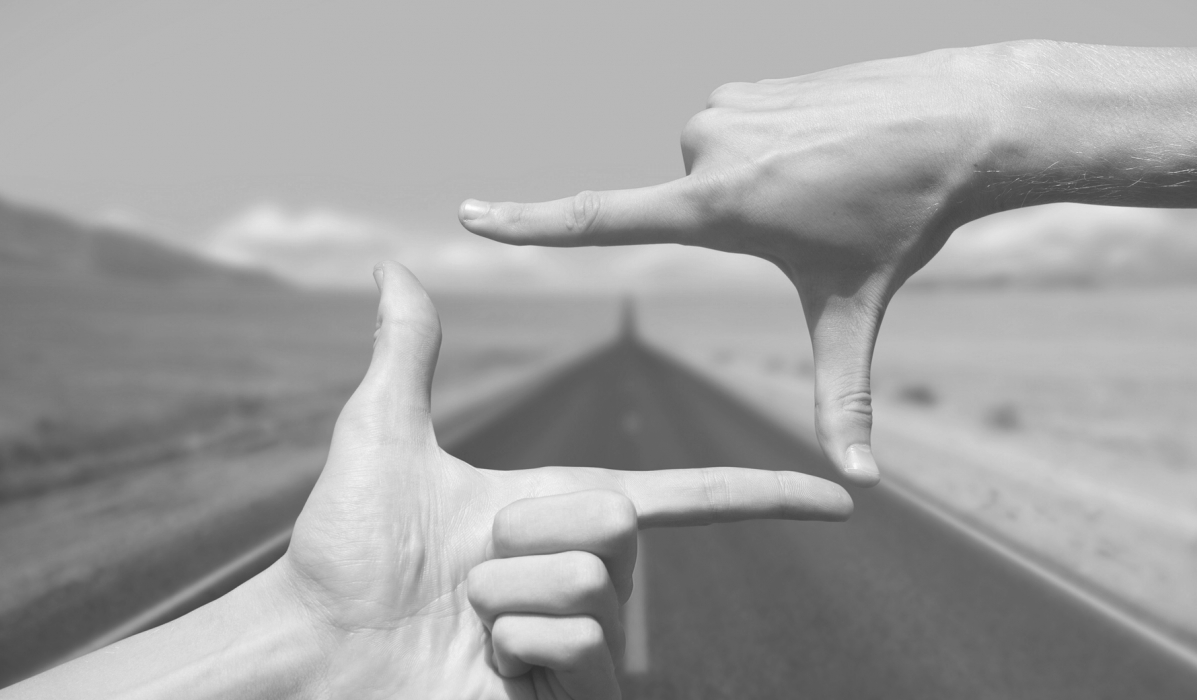
\includegraphics[width=\linewidth,valign=t]{frame.png}
\end{minipage}
\medskip

La photo est une matrice de taille 1920x1080. Chaque cellule contient un pixel coloré et occupe 3 octets (rouge, vert, bleu).
Le taux de compression d'une image est de l'ordre de 10.

\begin{itemize}
\item[$\cdot$] Quel est le rapport de taille entre la photo compressée et le message texte ?
\item[$\cdot$] Hors sujet : quel est le rapport de taille entre la photo d'un écran avec un programme Ada et le même programme Ada en tant que fichier texte (compter un texte de 2800 octets) ?
\item[$\cdot$] Combien de photos transmettez-vous par an ? (noter que chaque photo prise est probablement envoyée sur votre drive)
\item[$\cdot$] Exprimer le coût de transmission de ces photos en ecafé.
\end{itemize}

\lstinputlisting[language=Ada]{Ada/photo.ads}

\oldsection{Message vidéo}

Pour la vidéo, il convient de distinguer le son et l'image. Le traitement du son est similaire à la question~2. Pour les images,
prendre la même taille que les photos (1920x1080) et 25 images par seconde (25 fps).

\begin{itemize}
\item[$\cdot$] Calculer la taille de la vidéo non compressée, en octets. Rapporter à la taille du message texte.
\end{itemize}

La vidéo se compresse très bien en tolérant une baisse de qualité  (facteur de compression de 120).
%
\begin{itemize}
\item[$\cdot$] Calculer le rapport de taille entre un message vidéo compressé (avec le son) et un message texte.
\item[$\cdot$] Combien de messages vidéo envoyez-vous par an ? Estimer le coût en ecafé par an.
\end{itemize}

